
\section{Ejercicios}

\subsection{Ejercicios sobre disoluciones}

\begin{exercise}
    En 35 g de agua se disuelven 5 g de ácido clorhídrico. La densidad de la disolución resultante es \qty{1.06}{\g\per\cubic\centi\metre}. Halla la concentración de la disolución: a) en \% en masa , b) en \unit{\g\per\litre} , c) molaridad y d) normalidad.
    Sol: a) 12,5 \%,  b) \qty{132.5}{\g\per\litre},  c) \qty{3.63}{\M},  d) \qty{3.63}{\N}.

    \begin{solu}
        1. \textbf{Masa total:} $m_{dis} = 5\,\text{g (soluto)} + 35\,\text{g (disolvente)} = 40\,\text{g}$.

        a) \textbf{\% en masa:}
        \[ \% = \dfrac{\qty{5}{\g}}{\qty{40}{\g}} \cdot 100 = \mathbf{\textcolor{blue}{12,5 \%}} \]

        b) \textbf{Concentración en \unit{\g\per\litre}:}
        \[ C = \dfrac{\qty{5}{\g} \text{ sol.}}{\qty{40}{\g} \text{ dis.}} \cdot \dfrac{\qty{1.06}{\g} \text{ dis.}}{\qty{1}{\mL}} \cdot \dfrac{\qty{1000}{\mL}}{\qty{1}{\L}} = \mathbf{\textcolor{blue}{\qty{132.5}{\g\per\L}}} \]

        c) \textbf{Molaridad (M):} ($M_m HCl = \qty{36.5}{\g\per\mol}$)
        \[ M = \dfrac{\qty{132.5}{\g}}{\qty{1}{\L}} \cdot \dfrac{\qty{1}{\mol}}{\qty{36.5}{\g}} = \mathbf{\textcolor{blue}{\qty{3.63}{\M}}} \]

        d) \textbf{Normalidad (N):} Al ser $HCl$ monoprótico (un solo hidrógeno) ($v=1$), $N = M$. \textbf{\textcolor{blue}{\qty{3.63}{\N}}}.
    \end{solu}

\end{exercise}

\begin{exercise}
    Un ácido nítrico concentrado, de densidad \qty{1.405}{\g\per\cubic\centi\metre}, contiene 68,1 \% en masa de \ch{HNO3}. Calcula la molaridad, normalidad y molalidad de este ácido.
    Sol: \qty{15.18}{\M},  \qty{15.18}{\N} y  \qty{33.96}{\molal}.
    \begin{solu}
        Usamos factores de conversión sobre una base de \qty{1}{\L} de disolución:
        \[ M = \dfrac{\qty{1.405}{\g} \text{ dis.}}{\qty{1}{\mL} \text{ dis.}} \cdot \dfrac{\qty{1000}{\mL}}{\qty{1}{\L}} \cdot \dfrac{\qty{68.1}{\g} \text{ puro}}{\qty{100}{\g} \text{ dis.}} \cdot \dfrac{\qty{1}{\mol}}{\qty{63}{\g}} = \mathbf{\textcolor{blue}{\qty{15.18}{\M}}} \]
        $N = M \cdot 1 = \mathbf{\textcolor{blue}{\qty{15.18}{\N}}}$.

        Para la \textbf{molalidad}, en \qty{100}{\g} de disolución hay \qty{68.1}{\g} de soluto y \qty{31.9}{\g} de agua:
        \[ m = \dfrac{\qty{68.1}{\g} \text{ sol.}}{\qty{31.9}{\g} \text{ agua}} \cdot \dfrac{\qty{1000}{\g}}{\qty{1}{\kg}} \cdot \dfrac{\qty{1}{\mol}}{\qty{63}{\g}} = \mathbf{\textcolor{blue}{\qty{33.96}{\molal}}} \]
    \end{solu}

\end{exercise}

\begin{exercise}
    Calcula la fracción molar del metanol (\ch{CH3OH}) en una disolución acuosa \qty{0.1}{\M}. Sol: 1,79 . 10 3.
    \begin{solu}
        En una disolución acuosa diluida, el volumen de la disolución es aproximadamente el del agua ($\rho_{agua} \approx \qty{1}{\kg\per\L}$). En \qty{1}{\L} (\qty{1000}{\g}) de agua hay:
        \[ n_{agua} = \dfrac{\qty{1000}{\g}}{\qty{18}{\g\per\mol}} = \qty{55.55}{\mol} \]
        Moles de metanol = \qty{0.1}{\mol} (por definición de \qty{0.1}{\M}).
        \[ \chi_{metanol} = \dfrac{n_{sol}}{n_{sol} + n_{dis}} = \dfrac{0,1}{0,1 + 55,55} = \mathbf{\textcolor{blue}{1,79 \cdot 10^{-3}}} \]
    \end{solu}
\end{exercise}

\begin{exercise}
    Si \qty{9}{\L} de cloruro de hidrógeno, medidos a \qty{20}{\celsius} y \qty{750}{\mmhg}, se disuelven en el agua necesaria para dar \qty{290}{\mL} disolución, ¿cuál es la M de la disolución?.
    Sol: \qty{1.27}{\M}.

    \begin{solu}
        1. \textbf{Cálculo de moles de soluto (Gas):} Usamos $PV = nRT$.
        $P = \dfrac{750}{760} \unit{\atm} = \qty{0.987}{\atm}$; $V = \qty{9}{\L}$; $T = 20 + 273 = \qty{293}{\K}$.
        \[ n = \dfrac{P \cdot V}{R \cdot T} = \dfrac{\qty{0.987}{\atm} \cdot \qty{9}{\L}}{\qty{0.082}{\atm\L\per\mol\per\K} \cdot \qty{293}{\K}} = \qty{0.3694}{\mol} \]

        2. \textbf{Molaridad:} $V_{dis} = \qty{0.290}{\L}$.
        \[ M = \dfrac{\qty{0.3694}{\mol}}{\qty{0.290}{\L}} = \mathbf{\textcolor{blue}{\qty{1.27}{\M}}} \]
    \end{solu}
\end{exercise}

\begin{exercise}
    ¿Qué volumen de ácido nítrico con el 68\% de riqueza y \qty{1.4}{\g\per\cubic\centi\metre} de densidad se necesita para preparar \qty{3}{\L} de una disolución \qty{0.5}{\M} de ácido nítrico?.
    Sol: \qty{99.26}{\cc}

    \begin{solu}
        1. \textbf{Moles necesarios:} $n = \qty{3}{\L} \cdot \qty{0.5}{\mol\per\L} = \qty{1.5}{\mol}$.

        2. \textbf{Cálculo del volumen del ácido comercial:}
        \[ V = \qty{1.5}{\mol} \cdot \dfrac{\qty{63}{\g}}{\qty{1}{\mol}} \cdot \dfrac{\qty{100}{\g} \text{ dis.}}{\qty{68}{\g} \text{ puro}} \cdot \dfrac{\qty{1}{\mL} \text{ dis.}}{\qty{1.4}{\g} \text{ dis.}} = \mathbf{\textcolor{blue}{\qty{99.26}{\mL}}} \]
    \end{solu}
\end{exercise}

\begin{exercise}
    Disponemos de \qty{90}{\g} de cloruro de magnesio y queremos disolverlo en agua hasta obtener una disolución de concentración \qty{1.2}{\M}. ¿Qué volumen de disolución prepararemos?.
    Sol: \qty{0.787}{\L}.

    \begin{solu}
        1. \textbf{Moles de soluto ($MgCl_2$):} $M_m \approx 24.3 + 2(35.5) = \qty{95.3}{\g\per\mol}$.
        \[ n = \dfrac{\qty{90}{\g}}{\qty{95.3}{\g\per\mol}} = \qty{0.944}{\mol} \]

        2. \textbf{Volumen necesario:}
        \[ V = \dfrac{n}{M} = \dfrac{\qty{0.944}{\mol}}{\qty{1.2}{\mol\per\L}} = \mathbf{\textcolor{blue}{\qty{0.787}{\L}}} \]
    \end{solu}
\end{exercise}

\begin{exercise}
    Calcula la molaridad, normalidad, molalidad y fracción molar del soluto de una disolución de ácido sulfúrico de densidad \qty{1.198}{\g\per\cc} que contiene 27 \% de ácido sulfúrico en peso.
    Sol: \qty{3.3}{\M}, \qty{6.6}{\N},  \qty{3.78}{\molal} y 0,064.

    \begin{solu}
        Base: \qty{1}{\L} de disolución. $M_m \ch{H2SO4} = \qty{98}{\g\per\mol}$.

        a) \textbf{Molaridad:}
        \[ M = \dfrac{\qty{1198}{\g} \text{ dis.}}{\qty{1}{\L}} \cdot \dfrac{\qty{27}{\g} \text{ puro}}{\qty{100}{\g} \text{ dis.}} \cdot \dfrac{\qty{1}{\mol}}{\qty{98}{\g}} = \mathbf{\textcolor{blue}{\qty{3.3}{\M}}} \]

        b) \textbf{Normalidad:} Como tiene 2 hidrógenos: $N = 3.3 \cdot 2 = \mathbf{\textcolor{blue}{\qty{6.6}{\N}}}$.

        c) \textbf{Molalidad:} Masa agua en \qty{100}{\g} dis. = $100 - 27 = \qty{73}{\g}$.
        \[ m = \dfrac{\qty{27}{\g} \text{ sol.}}{\qty{73}{\g} \text{ agua}} \cdot \dfrac{\qty{1000}{\g}}{\qty{1}{\kg}} \cdot \dfrac{\qty{1}{\mol}}{\qty{98}{\g}} = \mathbf{\textcolor{blue}{\qty{3.78}{\molal}}} \]

        d) \textbf{Fracción molar ($\chi$):} $n_{sol} = \dfrac{27}{98} = \qty{0.2755}{\mol}$; $n_{agua} = \dfrac{73}{18} = \qty{4.055}{\mol}$.
        \[ \chi = \dfrac{0.2755}{0.2755 + 4.055} = \mathbf{\textcolor{blue}{0,064}} \]
    \end{solu}
\end{exercise}

\begin{exercise}
    ¿Cuál será la molaridad de una disolución de ácido nítrico preparada por dilución a \qty{500}{\mL}, de \qty{32}{\mL} de un ácido concentrado de densidad \qty{1.42}{\gpcc} y una riqueza de ácido nítrico de 69,5 \%?.
    Sol: \qty{1}{\M}.
    \begin{figure}[H]
        \centering
        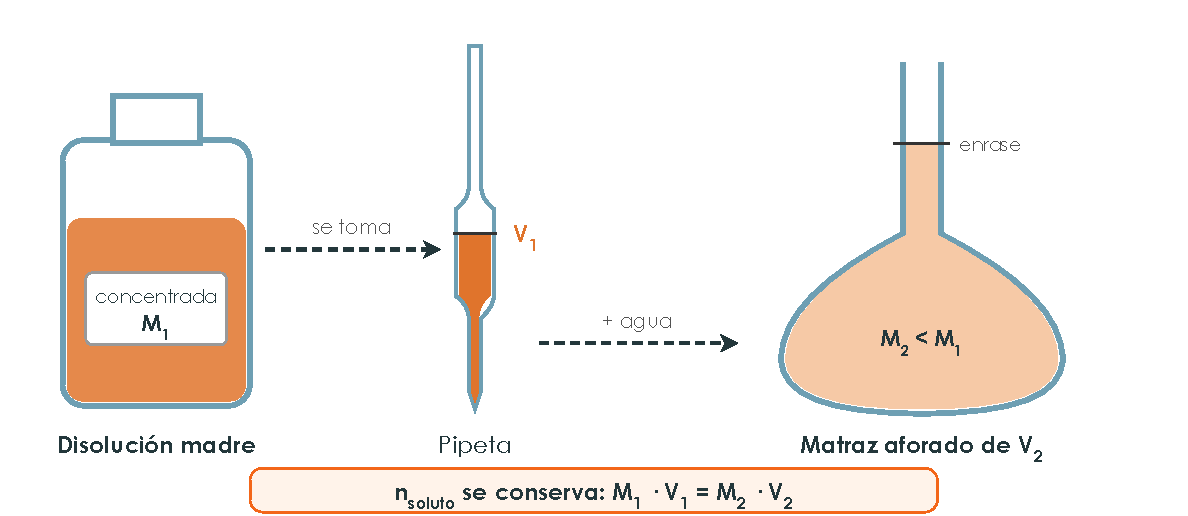
\includegraphics[width=0.75\linewidth]{FigurasSVG/UD0_Conocimientos_Basicos/pdf/UD0_E01_dilucion.pdf}
        \caption{Preparación de una disolución por dilución}
        \label{fig:dilucion}
    \end{figure}

    \begin{solu}
        1. \textbf{Moles en la porción de \qty{32}{\mL}:}
        \[ n = \qty{32}{\mL} \cdot \dfrac{\qty{1.42}{\g}}{\qty{1}{\mL}} \cdot \dfrac{69.5}{100} \cdot \dfrac{\qty{1}{\mol}}{\qty{63}{\g}} = \qty{0.501}{\mol} \]

        2. \textbf{Molaridad final:} Al diluir a \qty{500}{\mL} (\qty{0.5}{\L}):
        \[ M = \dfrac{\qty{0.501}{\mol}}{\qty{0.5}{\L}} = \mathbf{\textcolor{blue}{\qty{1}{\M}}} \]
    \end{solu}
\end{exercise}

\begin{exercise}
    Un litro de ácido clorhídrico del 35\% en masa y densidad \qty{1.18}{\gpcc}, debe diluirse de tal manera que se obtenga ácido al 20 \%. ¿ Qué cantidad de agua deberá añadirse?.
    Sol: \qty{885}{\mL}.

    \begin{solu}
        1. \textbf{Masa inicial de la disolución:} $m_1 = \qty{1000}{\mL} \cdot \qty{1.18}{\g\per\mL} = \qty{1180}{\g}$.

        2. \textbf{Masa de soluto (HCl):} $m_{sol} = \qty{1180}{\g} \cdot 0.35 = \qty{413}{\g}$.

        3. \textbf{Masa de la disolución final (20\%):} El soluto no cambia.
        \[ m_2 = \dfrac{\qty{413}{\g}}{0.20} = \qty{2065}{\g} \]

        4. \textbf{Agua añadida:} $m_{agua} = 2065 - 1180 = \mathbf{\textcolor{blue}{\qty{885}{\g}}} \rightarrow \mathbf{\textcolor{blue}{\qty{885}{\mL}}}$.
    \end{solu}
\end{exercise}

\begin{exercise}
    Calcula la M de una disolución preparada mezclando \qty{50}{\mL} de ácido sulfúrico \qty{0.136}{\M} con \qty{90}{\mL} de una disolución de ácido sulfúrico \qty{0.068}{\M}.
    Sol: \qty{0.092}{\M}.
    \begin{solu}
        1. \textbf{Moles totales:}
        $n_1 = \qty{0.050}{\L} \cdot \qty{0.136}{\mol\per\L} = \qty{0.0068}{\mol}$ \\
        $n_2 = \qty{0.090}{\L} \cdot \qty{0.068}{\mol\per\L} = \qty{0.00612}{\mol}$ \\
        $n_{tot} = \qty{0.01292}{\mol}$
        2. \textbf{Volumen total:} $V_{tot} = 50 + 90 = \qty{140}{\mL} = \qty{0.140}{\L}$.
        3. \textbf{Molaridad:}
        \[ M = \dfrac{\qty{0.01292}{\mol}}{\qty{0.140}{\L}} = \mathbf{\textcolor{blue}{\qty{0.092}{\M}}} \]
    \end{solu}
\end{exercise}

\begin{exercise}
    Una disolución de ácido acético al 10\% tiene \qty{1.055}{\gpcc} de densidad, se desea saber:
    a) ¿cuál es su molalidad?. b) si añadimos un litro de agua a \qty{500}{\cc} de la disolución anterior, ¿cuál es el \% en peso y la normalidad de la nueva disolución? Sol: \qty{1.55}{\molal} , 3,45 \%, \qty{0.58}{\N}
    \begin{solu}
        a) \textbf{Molalidad:} $M_m \approx \qty{60}{\g\per\mol}$. En \qty{100}{\g} dis.: \qty{10}{\g} sol. y \qty{90}{\g} agua.
        \[ m = \dfrac{\qty{10}{\g} \text{ sol.}}{\qty{90}{\g} \text{ agua}} \cdot \dfrac{\qty{1000}{\g}}{\qty{1}{\kg}} \cdot \dfrac{\qty{1}{\mol}}{\qty{60}{\g}} = \mathbf{\textcolor{blue}{\qty{1.85}{\molal}}} \]

        b) \textbf{Dilución:} En \qty{500}{\mL} (\qty{0.5}{\L}) iniciales: \\
        Masa dis. = $500 \cdot 1.055 = \qty{527.5}{\g}$. \\
        Masa soluto = $527.5 \cdot 0.10 = \qty{52.75}{\g}$. \\
        Añadimos \qty{1}{\L} (\qty{1000}{\g}) de agua: \\
        Masa final dis. = $527.5 + 1000 = \qty{1527.5}{\g}$. \\
        $\% \text{ peso} = \dfrac{52,75}{1527,5} \cdot 100 = \mathbf{\textcolor{blue}{3,45 \%}}$. \\
        Normalidad (suponiendo volúmenes aditivos $V \approx \qty{1.5}{\L}$): \\
        $n = 52.75 / 60 = \qty{0.879}{\mol}$. $M = 0.879 / 1.5 = \qty{0.58}{\M}$. Como es monoprótico, \textbf{\textcolor{blue}{\qty{0.58}{\N}}}.
    \end{solu}
\end{exercise}

\subsection{Ejercicios sobre gases}

\begin{exercise}
    Un neumático de una motocicleta tiene un volumen de 10 litros y se llena de aire a una presión de 3 atm, a 27ºC. Después de circular varias horas, la T se eleva a 57ºC y el volumen se supone invariable. Calcula: a) la presión que habrá en el neumático, b) el volumen del gas si la presión hubiera aumentado sin variar la T.
    Sol: a) \qty{3.3}{\atm}, b) \qty{9.09}{\L}.

    \begin{solu}
        Datos: $V_1 = \qty{10}{\L}$, $P_1 = \qty{3}{\atm}$, $T_1 = 27 + 273 = \qty{300}{\K}$. \\
        a) Presión a $T_2 = 57 + 273 = \qty{330}{\K}$ ($V$ cte):
        \[ P_2 = P_1 \cdot \dfrac{T_2}{T_1} = \qty{3}{\atm} \cdot \dfrac{\qty{330}{\K}}{\qty{300}{\K}} = \mathbf{\textcolor{blue}{\qty{3,3}{\atm}}} \]
        b) Volumen si $P_2 = \qty{3,3}{\atm}$ a $T_1$ cte:
        \[ V_2 = \dfrac{P_1 \cdot V_1}{P_2} = \dfrac{\qty{3}{\atm} \cdot \qty{10}{\L}}{\qty{3,3}{\atm}} = \mathbf{\textcolor{blue}{\qty{9,09}{\L}}} \]
    \end{solu}
\end{exercise}

\begin{exercise}
    Un volumen de \qty{2.38}{\litre} de un gas, medido a \qty{97}{\celsius} y \qty{720}{\mmhg}, tiene una masa de \qty{2.81}{\g}. Calcula la masa molecular de dicho gas.
    Sol: 37,8

    \begin{solu}
        Datos: $V = \qty{2,38}{\L}$, $T = \qty{370}{\K}$, $P = \dfrac{720}{760} = \qty{0,947}{\atm}$. \\
        Usamos $PV = nRT \Rightarrow M = \dfrac{mRT}{PV}$:
        \[ M = \dfrac{\qty{2,81}{\g} \cdot \qty{0,082}{\atm\L\per\mol\K} \cdot \qty{370}{\K}}{\qty{0,947}{\atm} \cdot \qty{2,38}{\L}} = \mathbf{\textcolor{blue}{\qty{37,8}{\g\per\mol}}} \]
    \end{solu}
\end{exercise}

\begin{exercise}
    Calcula la densidad del vapor del alcohol etílico cuando se encuentra en un recipiente cerrado: a) a \qty{0.8}{\atm} y \qty{37}{\celsius},  b) en c.n. .
    Sol: a) \qty{1.45}{\gpl},  b) \qty{2.05}{\gpl}.

    \begin{solu}
        $M_m = \qty{46}{\g\per\mol}$. \\
        a) $P = \qty{0,8}{\atm}$, $T = \qty{310}{\K}$:
        \[ d = \dfrac{P \cdot M}{R \cdot T} = \dfrac{0,8 \cdot 46}{0,082 \cdot 310} = \mathbf{\textcolor{blue}{\qty{1,45}{\g\per\L}}} \]
        b) c.n. ($P=1$, $T=273$):
        \[ d = \dfrac{1 \cdot 46}{0,082 \cdot 273} = \mathbf{\textcolor{blue}{\qty{2,05}{\g\per\L}}} \]
    \end{solu}
\end{exercise}

\begin{exercise}
    Sabiendo que la densidad de cierto gas a \qty{30}{\celsius} y \qty{310}{\mmhg} es de \qty{1.02}{\gpl}, calcula la masa molecular del gas.
    Sol: 62,1.
    \begin{solu}
        $P = \dfrac{310}{760} = \qty{0,408}{\atm}$, $T = \qty{303}{\K}$.
        \[ M = \dfrac{dRT}{P} = \dfrac{1,02 \cdot 0,082 \cdot 303}{0,408} = \mathbf{\textcolor{blue}{\qty{62,1}{\g\per\mol}}} \]
    \end{solu}
\end{exercise}

\begin{exercise}
    Un matraz de vidrio pesa vacío \qty{21.786}{\g}, lleno de nitrógeno pesa \qty{22.473}{\g} y lleno de un gas desconocido, en las mismas condiciones de p y T, con masa \qty{22.957}{\g}. Halla la masa molecular del gas. Sol: 47,7
    \begin{solu}
        $m_{N_2} = 22,473 - 21,786 = \qty{0,687}{\g}$. $m_{gas} = 22,957 - 21,786 = \qty{1,171}{\g}$. \\
        Como $n_{N_2} = n_{gas}$ en iguales $P, V, T$:
        \[ M_{gas} = M_{N_2} \cdot \dfrac{m_{gas}}{m_{N_2}} = 28 \cdot \dfrac{1,171}{0,687} = \mathbf{\textcolor{blue}{\qty{47,7}{\g\per\mol}}} \]
    \end{solu}
\end{exercise}

\begin{exercise}
    En un recipiente cerrado hay \qty{44}{\g} de dióxido de carbono y \qty{70}{\g} de nitrógeno a la presión total de \qty{0.5}{\atm}. Calcula la presión parcial de cada gas.
    Sol: \qty{0.143}{\atm} y \qty{0.357}{\atm}.
    \begin{solu}
        $n_{\ch{CO2}} = \dfrac{44}{44} = 1$; $n_{N_2} = \dfrac{70}{28} = 2,5$. $n_{tot} = \qty{3,5}{\mol}$.
        \[ P_{\ch{CO2}} = \dfrac{1}{3,5} \cdot 0,5 = \mathbf{\textcolor{blue}{\qty{0,143}{\atm}}} ; P_{N_2} = \dfrac{2,5}{3,5} \cdot 0,5 = \mathbf{\textcolor{blue}{\qty{0,357}{\atm}}} \]
    \end{solu}
\end{exercise}

\begin{exercise}
    Un recipiente de \qty{1}{\L} contiene a \qty{168}{\celsius} una mezcla gaseosa de \ch{H2} y de \ch{O2}, de presiones parciales 326 y 652 \unit{\mmhg} respectivamente. En esas condiciones se hace saltar la chispa eléctrica, produciéndose la explosión de la mezcla y alcanzándose una temperatura de  \qty{197}{\celsius}. Se pide: a) reacción que ha tenido lugar y la composición volumétrica o molar. b) presión final en el recipiente.
    Sol: a) 40 \% agua y 60 \% oxígeno. b) \qty{1.16}{\atm}.
    \begin{solu}
        Reacción: \ch{2 H2 + O2 -> 2 H2O}. $n \propto P$. \\
        $P_{H_2} = 326$; $P_{O_2} = 652$. El \ch{H2} es el limitante (necesita $652/2 = 326$). \\
        Sobran $652 - 163 = 489$ de \ch{O2}. Se forman 326 de \ch{H2O} vapor. \\
        $n_{tot_final} = 489 + 326 = 815$. Ajustamos por temperatura ($T_1 =\qty{441}{\kelvin} \rightarrow  T_2  = \qty{470}{\kelvin} $):
        \[ P_{f} = 815 \cdot \dfrac{470}{441} = \qty{868,5}{\mmHg} = \mathbf{\textcolor{blue}{\qty{1,14}{\atmosphere}}} \]
    \end{solu}
\end{exercise}

\begin{exercise}
    Si la densidad del nitrógeno líquido es \qty{1.25}{\gpcc}. a) ¿A qué volumen se reducirá 1 litro de nitrógeno gaseoso en c.n. al condensarse?. b) Calcula la fracción aproximada del volumen del gas que ocupan las moléculas (no considerar los huecos que hay entre las moléculas del líquido).
    Sol: a) \qty{1}{\cc},  b)  0,1 \%

    \begin{solu}
        1. \textbf{Moles de \ch{N2} en \qty{1}{\L} (c.n.):}
        \[ n = \dfrac{\qty{1}{\L}}{\qty{22.4}{\L\per\mol}} = \qty{0.0446}{\mol} \]

        2. \textbf{Masa de ese nitrógeno:} $M_m(\ch{N2}) = \qty{28}{\g\per\mol}$.
        \[ m = 0,0446 \cdot 28 = \qty{1.25}{\g} \]

        a) \textbf{Volumen líquido:} Con $\rho = \qty{1.25}{\g\per\cc}$:
        \[ V_{liq} = \dfrac{\qty{1.25}{\g}}{\qty{1.25}{\g\per\cc}} = \mathbf{\textcolor{blue}{\qty{1}{\cc}}} \]

        b) \textbf{Fracción del volumen ocupado por las moléculas:} Comparando el volumen líquido (donde las moléculas están prácticamente empaquetadas, sin huecos) frente al volumen gaseoso inicial:
        \[ \% = \dfrac{V_{liq}}{V_{gas}} \cdot 100 = \dfrac{\qty{1}{\cc}}{\qty{1000}{\cc}} \cdot 100 = \mathbf{\textcolor{blue}{0,1 \%}} \]
    \end{solu}
\end{exercise}

\begin{exercise}
    La composición volumétrica (molar) de una mezcla gaseosa es la siguiente: 30\% de metano, 50\% de dióxido de carbono y 20\% de monóxido de carbono. Si la presión total es de 2 atm ¿cuál es la presión parcial de cada uno de los gases?.
    Sol: 1,01 atm , 0,61 atm , 0,38 atm

    \begin{solu}
        En una mezcla de gases ideales, el \% en volumen (molar) coincide con la fracción molar $\chi_i$, y la presión parcial se calcula como $P_i = \chi_i \cdot P_{total}$.

        \[ P_{\ch{CH4}} = 0,30 \cdot \qty{2}{\atm} = \mathbf{\textcolor{blue}{\qty{0,6}{\atm}}} \]
        \[ P_{\ch{CO2}} = 0,50 \cdot \qty{2}{\atm} = \mathbf{\textcolor{blue}{\qty{1,0}{\atm}}} \]
        \[ P_{\ch{CO}} = 0,20 \cdot \qty{2}{\atm} = \mathbf{\textcolor{blue}{\qty{0,4}{\atm}}} \]

        (Los valores concuerdan, salvo el orden, con el enunciado: 1,0 atm para \ch{CO2}, 0,6 atm para \ch{CH4} y 0,4 atm para \ch{CO}).
    \end{solu}
\end{exercise}

\subsection{Fórmulas y estequiometría}

\begin{exercise}
    Halla el factor de conversión entre la u.m.a. y el gramo.
    \begin{solu}
        Por definición de mol y $N_A$:
        \[ 1 \text{ u.m.a.} = \dfrac{1}{N_A} \si{\g} = \dfrac{1}{6,022 \cdot 10^{23}} = \mathbf{\textcolor{blue}{1,66 \cdot 10^{-24} \si{\g}}} \]
    \end{solu}
\end{exercise}

\begin{exercise}
    ¿Cuántos moles de átomos y cuántos átomos de hidrógeno hay en \qty{0.04}{\g} de sulfuro de hidrógeno?.
    \begin{solu}
        $M(\ch{H2S}) = \qty{34}{\g\per\mol}$.
        \[ n_{at\_H} = \qty{0,04}{\g \ch{H2S}} \cdot \dfrac{1 \text{ mol}}{34 \si{\g}} \cdot \dfrac{2 \text{ mol at H}}{1 \text{ mol \ch{H2S}}} = \mathbf{\textcolor{blue}{2,35 \cdot 10^{-3} \text{ moles}}} \]
        \[ At\_H = 2,35 \cdot 10^{-3} \cdot 6,022 \cdot 10^{23} = \mathbf{\textcolor{blue}{1,41 \cdot 10^{21} \text{ átomos}}} \]
    \end{solu}
\end{exercise}

\begin{exercise}
    Para obtener óxido de estaño (IV) se han hecho reaccionar \qty{8.32}{\g} de estaño con \qty{2.51}{\g} de oxígeno. ¿Qué cantidad de óxido se formará?. Sol: \qty{10.55}{\g}
    \begin{solu}
        Ley de conservación de la masa:
        \[ \text{Masa óxido} = 8,32 + 2,51 = \mathbf{\textcolor{blue}{\qty{10,83}{\g}}} \]
        Nota: Según el ajuste estequiométrico \ch{Sn + O2 -> SnO2}, si reaccionan proporciones exactas es la suma.
    \end{solu}
\end{exercise}

\begin{exercise}
    Se desea formar un compuesto en el que entren dos átomos de cromo por cada tres de azufre. Si disponemos de 6 gramos de azufre, ¿cuántos gramos de cromo habrán de utilizarse?. Sol: \qty{6.5}{\g}
    \begin{solu}
        Fórmula \ch{Cr2S3}.
        \[ m_{\ch{Cr}} = \qty{6}{\g \ch{S}} \cdot \dfrac{1 \si{\mol \ch{S}}}{32 \si{\g \ch{S}}} \cdot \dfrac{2 \si{\mol \ch{Cr}}}{3 \si{\mol \ch{S}}} \cdot \dfrac{52 \si{\g \ch{Cr}}}{1 \si{\mol \ch{Cr}}} = \mathbf{\textcolor{blue}{\qty{6,5}{\g}}} \]
    \end{solu}
\end{exercise}

\begin{exercise}
    Si para formar un cloruro de titanio, este y el cloro entran en una relación en peso 1:3, ¿cuál será la fórmula del cloruro? Sol: \ch{TiCl4}
    \begin{solu}
        Tomamos como base \qty{1}{\g} de titanio y \qty{3}{\g} de cloro (relación en peso 1:3). $M_m(\ch{Ti}) = \qty{47.9}{\g\per\mol}$; $M_m(\ch{Cl}) = \qty{35.5}{\g\per\mol}$.
        \[ n_{\ch{Ti}} = \dfrac{1}{47,9} = 0,0209 \si{\mol} \qquad n_{\ch{Cl}} = \dfrac{3}{35,5} = 0,0845 \si{\mol} \]
        Dividiendo por el menor de los dos:
        \[ \dfrac{n_{\ch{Ti}}}{0,0209} = 1 \qquad \dfrac{n_{\ch{Cl}}}{0,0209} = 4,04 \approx 4 \]
        Por tanto la fórmula del cloruro es \(\mathbf{\textcolor{blue}{\ch{TiCl4}}}\).
    \end{solu}
\end{exercise}

\begin{exercise}
    Un compuesto tiene la siguiente composición centesimal: N = 14,29 \% , H = 4,11 \% , Mo = 48,95 \% , O = 32,65  \%. Calcula su fórmula. Sol: (NH4)2 MoO4
    \begin{solu}
        Tomamos como base \qty{100}{\g} de compuesto. Masas atómicas: $N=14$, $H=1$, $Mo=95,9$, $O=16$.
        \[ n_N = \dfrac{14,29}{14} = 1,021 \qquad n_H = \dfrac{4,11}{1} = 4,11 \]
        \[ n_{Mo} = \dfrac{48,95}{95,9} = 0,5105 \qquad n_O = \dfrac{32,65}{16} = 2,041 \]
        Dividiendo todos por el menor ($n_{Mo} = 0,5105$):
        \[ N: \dfrac{1,021}{0,5105} \approx 2 \quad H: \dfrac{4,11}{0,5105} \approx 8 \quad Mo: 1 \quad O: \dfrac{2,041}{0,5105} \approx 4 \]
        La fórmula empírica es \(N_2H_8MoO_4\), que se reagrupa como el molibdato de amonio:
        \[ \mathbf{\textcolor{blue}{\ch{(NH4)2MoO4}}} \]
    \end{solu}
\end{exercise}

\begin{exercise}
    La fórmula de la vitamina C es \ch{C6H8O6}. ¿Cuál es su composición centesimal?.
    \begin{solu}
        $M = \qty{176}{\g\per\mol}$. \\
        $\%C = \dfrac{72}{176} = \mathbf{\textcolor{blue}{40,9 \%}}$; $\%H = \dfrac{8}{176} = \mathbf{\textcolor{blue}{4,5 \%}}$; $\%O = \dfrac{96}{176} = \mathbf{\textcolor{blue}{54,6 \%}}$.
    \end{solu}
\end{exercise}

\begin{exercise}
    La nicotina es un producto compuesto por un 74\% de Carbono, 8,7\% de hidrógeno y 17,3\% de nitrógeno. ¿Qué porcentaje de los átomos de la nicotina son átomos de nitrógeno?. Sol: 7,7\%
    \begin{solu}
        Tomamos como base \qty{100}{\g} de nicotina. Masas atómicas: $C=12$, $H=1$, $N=14$.
        \[ n_C = \dfrac{74}{12} = 6,167 \qquad n_H = \dfrac{8,7}{1} = 8,7 \qquad n_N = \dfrac{17,3}{14} = 1,236 \]
        El \% de átomos de nitrógeno es el cociente entre sus moles y el total de moles de átomos:
        \[ n_{tot} = 6,167 + 8,7 + 1,236 = 16,10 \si{\mol\ at.} \]
        \[ \%N_{at} = \dfrac{1,236}{16,10} \cdot 100 = \mathbf{\textcolor{blue}{7,7 \%}} \]
    \end{solu}
\end{exercise}

\begin{exercise}
    La masa molar de la aspirina es 180,2 g. Si la composición centesimal es 60 \% de C, 4,5 \% de H, y 35,5 \% de O. ¿Cuáles son las fórmulas empírica y molecular?. Sol: \ch{C9H8O4}
    \begin{solu}
        Tomamos como base \qty{100}{\g}. Masas atómicas: $C=12$, $H=1$, $O=16$.
        \[ n_C = \dfrac{60}{12} = 5 \qquad n_H = \dfrac{4,5}{1} = 4,5 \qquad n_O = \dfrac{35,5}{16} = 2,22 \]
        Dividiendo por el menor ($n_O = 2,22$):
        \[ C: \dfrac{5}{2,22} = 2,25 \qquad H: \dfrac{4,5}{2,22} = 2,03 \qquad O: 1 \]
        Como no son enteros, multiplicamos por 4: $C = 9$, $H = 8,1 \approx 8$, $O = 4$. \\
        \textbf{Fórmula empírica:} \(\ch{C9H8O4}\), con masa $M_{emp} = 9(12)+8(1)+4(16) = \qty{180}{\g\per\mol}$.

        Como $M_{emp} \approx M_{molecular} = \qty{180.2}{\g\per\mol}$, la fórmula molecular coincide con la empírica:
        \[ \mathbf{\textcolor{blue}{\ch{C9H8O4}}} \]
    \end{solu}
\end{exercise}


\begin{exercise}
    En 4,83 g de un hidrocarburo gaseoso hay 4,14 g de carbono. Halla su fórmula molecular si esos gramos del mismo, a 18ºC y 740 mm de Hg, ocupan un volumen de 2,82 litros. Sol: C3H6
    \begin{solu}
        1. \textbf{Composición:} $m_H = 4,83 - 4,14 = \qty{0,69}{\g}$.
        \[ n_C = \dfrac{4,14}{12} = 0,345 \si{\mol} \qquad n_H = \dfrac{0,69}{1} = 0,69 \si{\mol} \]
        Dividiendo por el menor: $C = 1$, $H = 2 \Rightarrow$ fórmula empírica \ch{CH2} ($M_{emp} = \qty{14}{\g\per\mol}$).

        2. \textbf{Masa molecular real:} $P = \dfrac{740}{760} = \qty{0,974}{\atm}$; $T = 18+273 = \qty{291}{\K}$.
        \[ M = \dfrac{mRT}{PV} = \dfrac{4,83 \cdot 0,082 \cdot 291}{0,974 \cdot 2,82} = \qty{42,03}{\g\per\mol} \]

        3. \textbf{Fórmula molecular:} $n = \dfrac{42,03}{14} \approx 3 \Rightarrow$
        \[ \mathbf{\textcolor{blue}{\ch{C3H6}}} \]
    \end{solu}
\end{exercise}

\begin{exercise}
    El yeso es sulfato cálcico hidratado. a) Si al calentar 3,273 g de yeso se convierten en 2,588 g de sulfato cálcico anhidro, calcula la fórmula del yeso. b) ¿ Cuántos moles de agua hay en 25 g de yeso?. Sol: a) CaSO4 · 2H2O ,  b)
    \begin{solu}
        a) \textbf{Fórmula del yeso:} Al calentar se pierde el agua de hidratación:
        \[ m_{\ch{H2O}} = 3,273 - 2,588 = \qty{0,685}{\g} \]
        \[ n_{\ch{CaSO4}} = \dfrac{2,588}{136} = 0,01903 \si{\mol} \qquad n_{\ch{H2O}} = \dfrac{0,685}{18} = 0,0381 \si{\mol} \]
        \[ \dfrac{n_{\ch{H2O}}}{n_{\ch{CaSO4}}} = \dfrac{0,0381}{0,01903} \approx 2 \Rightarrow \mathbf{\textcolor{blue}{\ch{CaSO4.2H2O}}} \]

        b) \textbf{Moles de agua en \qty{25}{\g} de yeso:} $M_m(\ch{CaSO4.2H2O}) = 136 + 36 = \qty{172}{\g\per\mol}$.
        \[ n_{yeso} = \dfrac{25}{172} = 0,1453 \si{\mol} \]
        Como hay 2 moles de agua por mol de yeso:
        \[ n_{\ch{H2O}} = 2 \cdot 0,1453 = \mathbf{\textcolor{blue}{0,291 \si{\mol}}} \]
    \end{solu}
\end{exercise}

\begin{exercise}
    Una muestra de 1,20 g de un compuesto que contiene solo carbono e hidrógeno, ardió completamente en exceso de oxígeno, dando 3,6 g de CO2 y 1,96 g de H2O. Calcula la fórmula empírica del compuesto. Sol: C3H8.
    \begin{figure}[H]
        \centering
        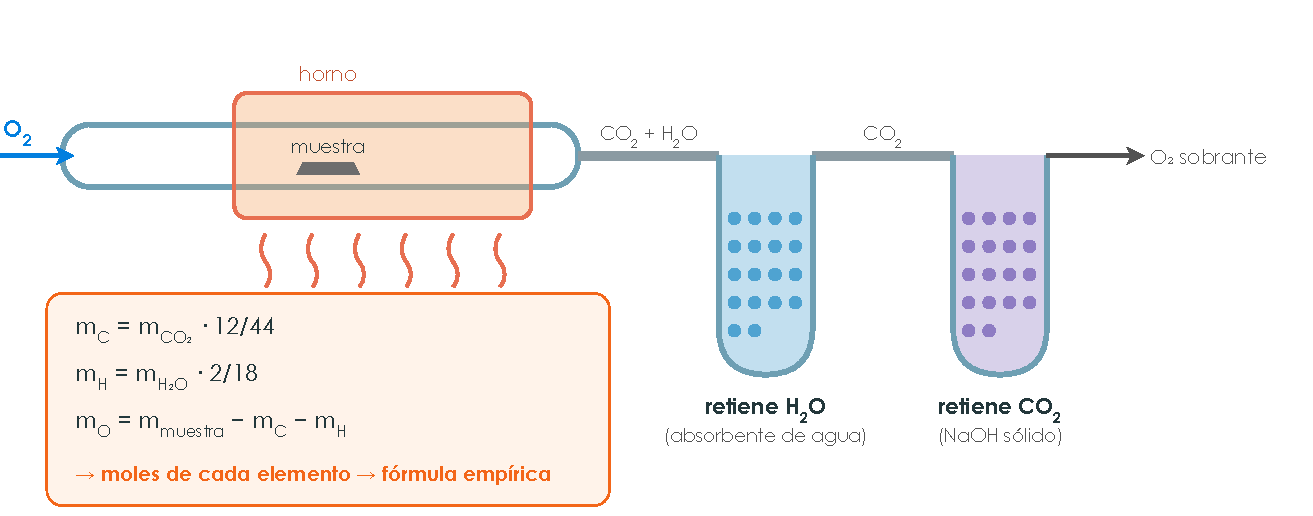
\includegraphics[width=0.85\linewidth]{FigurasSVG/UD0_Conocimientos_Basicos/pdf/UD0_E03_analisis_combustion.pdf}
        \caption{Análisis elemental por combustión}
        \label{fig:analisis-combustion}
    \end{figure}
    \begin{solu}
        \[ m_C = 3,6 \si{\g \ch{CO2}} \cdot \dfrac{12}{44} = \qty{0,982}{\g} \qquad m_H = 1,96 \si{\g \ch{H2O}} \cdot \dfrac{2}{18} = \qty{0,218}{\g} \]
        Comprobamos: $0,982 + 0,218 = \qty{1,20}{\g}$, coincide con la masa inicial (no hay oxígeno en el compuesto).
        \[ n_C = \dfrac{0,982}{12} = 0,0818 \si{\mol} \qquad n_H = \dfrac{0,218}{1} = 0,218 \si{\mol} \]
        Dividiendo por el menor:
        \[ C: \dfrac{0,0818}{0,0818} = 1 \qquad H: \dfrac{0,218}{0,0818} = 2,66 \]
        Multiplicando por 3 para obtener enteros: $C = 3$, $H = 8$. Fórmula empírica:
        \[ \mathbf{\textcolor{blue}{\ch{C3H8}}} \]
    \end{solu}
\end{exercise}

\begin{exercise}
    Un compuesto A se descompone por el calor formando un compuesto B y dióxido de carbono. Al calentar 300 g de A se obtuvieron 132 g de CO2 y se sabe que B tiene un 28\%  de O. ¿ Cuál será el porcentaje de O que contiene el compuesto A?. Sol: 47,68 \%
    \begin{solu}
        1. \textbf{Masa de B:} Por conservación de la masa, $A \rightarrow B + CO_2$:
        \[ m_B = 300 - 132 = \qty{168}{\g} \]

        2. \textbf{Masa de oxígeno en cada fragmento:}
        \[ m_{O(\ch{CO2})} = 132 \si{\g} \cdot \dfrac{32}{44} = \qty{96}{\g} \]
        \[ m_{O(B)} = 168 \si{\g} \cdot 0,28 = \qty{47,04}{\g} \]

        3. \textbf{Masa total de oxígeno en A y su porcentaje:}
        \[ m_{O(A)} = 96 + 47,04 = \qty{143,04}{\g} \]
        \[ \%O_A = \dfrac{143,04}{300} \cdot 100 = \mathbf{\textcolor{blue}{47,68 \%}} \]
    \end{solu}
\end{exercise}

\begin{exercise}
    Por tostación del sulfuro de cinc se obtiene el óxido del metal y se desprende dióxido de azufre. Si se dispone de 8,5 kg de sulfuro:
    a) ¿Qué cantidad de óxido se producirá?. b) ¿Con qué cantidad de oxígeno reacciona?
    Sol: a)  7.104 g de ZnO ; b) 4.189 g de oxígeno

    \begin{solu}
        \textbf{Reacción ajustada:} \ch{2 ZnS + 3 O2 -> 2 ZnO + 2 SO2}.

        1. \textbf{Moles de \ch{ZnS}:} $M_m(\ch{ZnS}) = 65,4 + 32 = \qty{97,4}{\g\per\mol}$.
        \[ n_{\ch{ZnS}} = \dfrac{8500}{97,4} = \qty{87,27}{\mol} \]

        a) \textbf{Masa de \ch{ZnO}:} Relación 1:1 con \ch{ZnS}. $M_m(\ch{ZnO}) = \qty{81,4}{\g\per\mol}$.
        \[ m_{\ch{ZnO}} = 87,27 \cdot 81,4 = \mathbf{\textcolor{blue}{\qty{7104}{\g}}} \]

        b) \textbf{Masa de \ch{O2}:} Relación 2:3 con \ch{ZnS}.
        \[ n_{\ch{O2}} = 87,27 \cdot \dfrac{3}{2} = \qty{130,9}{\mol} \]
        \[ m_{\ch{O2}} = 130,9 \cdot 32 = \mathbf{\textcolor{blue}{\qty{4189}{\g}}} \]
    \end{solu}
\end{exercise}

\begin{exercise}
    ¿ Qué masa de cloruro de plata puede obtenerse a partir de la reacción de 99,8 g de nitrato de plata con 35,4 g de cloruro de sodio?. Sol: 84,4 g
    \begin{solu}
        \textbf{Reacción:} \ch{AgNO3 + NaCl -> AgCl + NaNO3}.

        1. \textbf{Moles de cada reactivo:} $M_m(\ch{AgNO3}) = \qty{170}{\g\per\mol}$; $M_m(\ch{NaCl}) = \qty{58,5}{\g\per\mol}$.
        \[ n_{\ch{AgNO3}} = \dfrac{99,8}{170} = 0,587 \si{\mol} \qquad n_{\ch{NaCl}} = \dfrac{35,4}{58,5} = 0,605 \si{\mol} \]

        2. \textbf{Reactivo limitante:} Relación estequiométrica 1:1, luego \ch{AgNO3} (0,587 mol) es el limitante.

        3. \textbf{Masa de \ch{AgCl}:} $M_m(\ch{AgCl}) = \qty{143,4}{\g\per\mol}$.
        \[ m_{\ch{AgCl}} = 0,587 \cdot 143,4 = \mathbf{\textcolor{blue}{\qty{84,2}{\g}}} \]
    \end{solu}
\end{exercise}

\begin{exercise}
    ¿Cuántos \unit{\ml} de ácido clorhídrico del 25\% en peso y densidad \qty{0.91}{\gpml}  son necesarios para neutralizar \qty{32}{\g} de \ch{Ca(OH)2}. Sol: \qty{138.6}{\mL}
    \begin{solu}
        \ch{Ca(OH)2 + 2 HCl -> CaCl2 + 2 H2O}.
        \[ V = 32 \si{\g \ch{Ca(OH)2}} \cdot \dfrac{1 \si{\mol}}{74} \cdot \dfrac{2 \si{\mol \ch{HCl}}}{1 \si{\mol \ch{base}}} \cdot \dfrac{36,5 \si{\g}}{1 \si{\mol}} \cdot \dfrac{100 \si{\g \text{ dis.}}}{25 \si{\g \text{ ac.}}} \cdot \dfrac{1 \si{\mL}}{0,91 \si{\g}} = \mathbf{\textcolor{blue}{\qty{138,6}{\mL}}} \]
    \end{solu}
\end{exercise}

\begin{exercise}
    a) ¿Cuántos litros de oxígeno, medido en c.n., se necesitan para quemar \qty{36}{\g} de butano?. b) ¿Cuántos litros de \ch{CO2}, medidos en c.n., y cuántos gramos de agua se formarán?. Sol: a) \qty{90.4}{\L} de \ch{O}2. b) \qty{55.61}{\L} de \ch{CO2} y \qty{55.9}{\g} de agua.
    \begin{solu}
        1. \textbf{Reacción ajustada:} \( \ch{C4H10 + 13/2 O2 -> 4 CO2 + 5 H2O} \). \\
        2. \textbf{Moles de butano:} \( M(\ch{C4H10}) = \qty{58}{\g\per\mol} \). \\
        \( n = \dfrac{36}{58} = \qty{0,6207}{\mol} \). \\
        3. \textbf{Apartado a):} \\
        \( n_{\ch{O2}} = 0,6207 \cdot 6,5 = \qty{4,034}{\mol} \). \\
        \( V_{\ch{O2}} = 4,034 \si{\mol} \cdot 22,4 \si{\L\per\mol} = \textbf{\textcolor{blue}{\qty{90,37}{\L}}} \). \\
        4. \textbf{Apartado b):} \\
        \( V_{\ch{CO2}} = 0,6207 \cdot 4 \cdot 22,4 = \textbf{\textcolor{blue}{\qty{55,61}{\L}}} \). \\
        \( m_{\ch{H2O}} = 0,6207 \cdot 5 \cdot 18 = \textbf{\textcolor{blue}{\qty{55,86}{\g}}} \).
    \end{solu}

\end{exercise}

\begin{exercise}
    Halla el volumen de hidrógeno medido sobre agua, a \qty{25}{\celsius} y \qty{750}{\mmhg}, que se desprende al calentar \qty{1.52}{\g} de silicio con disolución de sosa cáustica, sabiendo que la presión de vapor del agua a \qty{25}{\celsius} es de \qty{23.8}{\mmhg} y que la reacción que tiene lugar es:
    \begin{reaction*}
        Si + 4 NaOH ->2 H2 + Na4SiO4
    \end{reaction*}
    Sol: \qty{2.77}{\L}
    \begin{figure}[H]
        \centering
        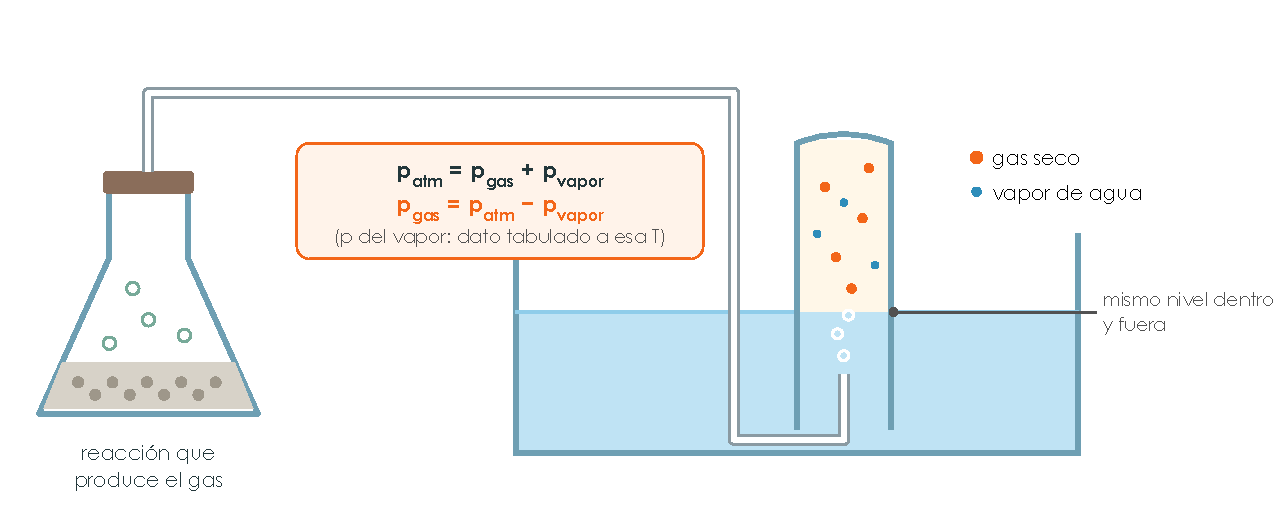
\includegraphics[width=0.8\linewidth]{FigurasSVG/UD0_Conocimientos_Basicos/pdf/UD0_E02_gas_sobre_agua.pdf}
        \caption{Gas recogido sobre agua}
        \label{fig:gas-sobre-agua}
    \end{figure}

    \begin{solu}
        1. \textbf{Moles de Si:} \( M(\text{Si}) = \qty{28,1}{\g\per\mol} \). \\
        \( n_{\text{Si}} = \dfrac{1,52}{28,1} = \qty{0,0541}{\mol} \). \\
        2. \textbf{Moles de \( \ch{H2} \):} Por estequiometría (1:2), \( n_{\ch{H2}} = 0,0541 \cdot 2 = \qty{0,1082}{\mol} \). \\
        3. \textbf{Presión del gas seco:} \( P_{\ch{H2}} = P_{total} - P_v = 750 - 23,8 = \qty{726,2}{\mmHg} = \qty{0,9555}{\atm} \). \\
        4. \textbf{Cálculo del volumen:} \\
        \( V = \dfrac{nRT}{P} = \dfrac{0,1082 \cdot 0,082 \cdot 298}{0,9555} = \textbf{\textcolor{blue}{\qty{2,77}{\L}}} \).
    \end{solu}

\end{exercise}

\begin{exercise}
    Halla la pureza de una muestra de sulfato de amonio, de la que tomados \qty{13.162}{\g} y tratados con exceso de sosa cáustica hacen desprender \qty{3.77}{\L}de amoniaco, medidos a \qty{18}{\celsius} y \qty{742}{\mmhg}, si además se origina sulfato de sodio y agua. Sol: 77,3\%

    \begin{solu}
        1. \textbf{Reacción:} \( \ch{(NH4)2SO4 + 2 NaOH -> 2 NH3 + Na2SO4 + 2 H2O} \). \\
        2. \textbf{Moles de \( \ch{NH3} \):} \( P = \dfrac{742}{760} = \qty{0,9763}{\atm} \); \( T = \qty{291}{\K} \). \\
        \( n_{\ch{NH3}} = \dfrac{0,9763 \cdot 3,77}{0,082 \cdot 291} = \qty{0,1544}{\mol} \). \\
        3. \textbf{Masa de \( \ch{(NH4)2SO4} \) pura:} (Relación 1:2) \\
        \( n_{sulfate} = \dfrac{0,1544}{2} = \qty{0,0772}{\mol} \). \\
        \( m_{puro} = 0,0772 \cdot 132,1 = \qty{10,198}{\g} \). \\
        4. \textbf{Pureza:} \( \% = \dfrac{10,198}{13,162} \cdot 100 = \textbf{\textcolor{blue}{77,5 \%}} \).
    \end{solu}

\end{exercise}

\begin{exercise}
    Calcula la pureza de una muestra de carburo cálcico (\ch{CaC2}) sabiendo que al tratar \qty{2.056}{\g} de carburo con agua se obtienen \qty{656}{\cc} de acetileno medidos sobre agua a \qty{22}{\celsius} y \qty{748}{\mmhg}. La presión de vapor del agua a \qty{22}{\celsius} es de \qty{19.8}{\mmhg}.
    \begin{reaction*}
        CaC2 + H2O -> C2H2 + Ca(OH)2.
    \end{reaction*}
    Sol: 81 \%
    \begin{solu}
        1. \textbf{Presión gas seco:} \( P = 748 - 19,8 = \qty{728,2}{\mmHg} = \qty{0,958}{\atm} \). \\
        2. \textbf{Moles de \( \ch{C2H2} \):} \( T = \qty{295}{\K} \); \( V = \qty{0,656}{\L} \). \\
        \( n = \dfrac{0,958 \cdot 0,656}{0,082 \cdot 295} = \qty{0,026}{\mol} \). \\
        3. \textbf{Masa de \( \ch{CaC2} \) pura:} (Relación 1:1) \\
        \( m_{puro} = 0,026 \si{\mol} \cdot 64,1 \si{\g\per\mol} = \qty{1,666}{\g} \). \\
        4. \textbf{Pureza:} \( \% = \dfrac{1,666}{2,056} \cdot 100 = \textbf{\textcolor{blue}{81,03 \%}} \).
    \end{solu}

\end{exercise}

\begin{exercise}
    Calcula la cantidad de caliza cuya riqueza en carbonato cálcico es del 85,3\%, que se necesita para obtener, por reacción con un exceso de ácido clorhídrico, \qty{10}{\L} de dióxido de carbono, medido a \qty{18}{\celsius} y \qty{752}{\mmhg}. Sol: \qty{48.6}{\g}
    \begin{solu}
        1. \textbf{Moles de \( \ch{CO2} \):} \( P = \dfrac{752}{760} = \qty{0,9895}{\atm} \); \( T = \qty{291}{\K} \). \\
        \( n = \dfrac{0,9895 \cdot 10}{0,082 \cdot 291} = \qty{0,415}{\mol} \). \\
        2. \textbf{Masa de \( \ch{CaCO3} \):} \( m = 0,415 \si{\mol} \cdot 100 \si{\g\per\mol} = \qty{41,5}{\g} \). \\
        3. \textbf{Masa de caliza:} \\
        \( m_{caliza} = \dfrac{41,5}{0,853} = \textbf{\textcolor{blue}{\qty{48,65}{\g}}} \).
    \end{solu}
\end{exercise}

\begin{exercise}
    ¿Cuántos gramos de cobre se obtendrán cuando el gas hidrógeno obtenido al hacer reaccionar \qty{41.6}{\g} de Al con un exceso de cloruro de hidrógeno se hace pasar sobre una cantidad en exceso de \ch{CuO}?. Las reacciones químicas son:
    \begin{reaction*}
        Al + HCl -> H2 + AlCl3
    \end{reaction*}
    \begin{reaction*}
        H2 + CuO -> Cu + H2O
    \end{reaction*}
    Sol: \qty{147}{\g}

    \begin{solu}
        1. \textbf{Moles de Al:} \( n = \dfrac{41,6}{27} = \qty{1,541}{\mol} \). \\
        2. \textbf{Moles de \( \ch{H2} \):} Ajuste \( \ch{2 Al + 6 HCl -> 2 AlCl3 + 3 H2} \). \\
        \( n_{\ch{H2}} = 1,541 \cdot \dfrac{3}{2} = \qty{2,3115}{\mol} \). \\
        3. \textbf{Moles de Cu:} Ajuste \( \ch{H2 + CuO -> Cu + H2O} \) (Relación 1:1). \\
        \( n_{\text{Cu}} = \qty{2,3115}{\mol} \). \\
        4. \textbf{Masa de Cu:} \( m = 2,3115 \si{\mol} \cdot 63,54 \si{\g\per\mol} = \textbf{\textcolor{blue}{\qty{146,87}{\g}}} \).
    \end{solu}

\end{exercise}

\begin{exercise}
    Una determinada cantidad de tricloruro de hierro ha sido oxidada completamente y todo el cloro se ha desprendido en forma de cloro. Este cloro gaseoso se ha empleado para transformar silicio en tetracloruro de silicio. Se han producido un total de \qty{7.44}{\mol} de tetracloruro de silicio. ¿Cuántos moles de tricloruro de hierro fueron oxidados?.
    \begin{reaction*}
        FeCl3 + O2 -> Cl2 + Fe2O3
    \end{reaction*}
    \begin{reaction*}
        Cl2 + Si -> SiCl4
    \end{reaction*}
    Sol: 9,92 moles
    \begin{solu}
        1. \textbf{Relación \( \ch{SiCl4} \) y \( \ch{Cl2} \):} \( \ch{Si + 2 Cl2 -> SiCl4} \). \\
        \( n_{\ch{Cl2}} = 7,44 \cdot 2 = \qty{14,88}{\mol} \). \\
        2. \textbf{Relación \( \ch{Cl2} \) y \( \ch{FeCl3} \):} \( \ch{4 FeCl3 + 3 O2 -> 2 Fe2O3 + 6 Cl2} \). \\
        Factor: \( 4 \si{\mol} \ch{FeCl3} \) producen \( 6 \si{\mol} \ch{Cl2} \). \\
        3. \textbf{Cálculo:} \\
        \( n_{\ch{FeCl3}} = 14,88 \si{\mol \ch{Cl2}} \cdot \dfrac{4 \si{\mol \ch{FeCl3}}}{6 \si{\mol \ch{Cl2}}} = \textbf{\textcolor{blue}{\qty{9,92}{\mol}}} \).
    \end{solu}

\end{exercise}

\begin{exercise}
    Se hace reaccionar 200 g de piedra caliza, que contiene un 60\% de carbonato cálcico con 200 cc de una disolución de ácido clorhídrico, de una concentración del 30\% (en peso) y densidad 1,15 g/ml. El proceso transcurre a 17ºC y 740 mmHg. Calcula: a) La masa de cloruro cálcico obtenido. b) el volumen de dióxido de carbono producido en las condiciones de la reacción. Sol: a) 104,9 g ,  b) 23,1 litros
    \begin{solu}
        \ch{CaCO3 + 2 HCl -> CaCl2 + CO2 + H2O}. \\
        $n_{\ch{CaCO3}} = \dfrac{200 \cdot 0,6}{100} = \qty{1,2}{\mol}$. $n_{\ch{HCl}} = \dfrac{200 \cdot 1,15 \cdot 0,3}{36,5} = \qty{1,89}{\mol}$. \\
        Limitante: \ch{HCl} (necesitaría 2,4 moles para todo el carbonato). \\
        a) $m_{\ch{CaCl2}} = \dfrac{1,89}{2} \cdot 111 = \mathbf{\textcolor{blue}{\qty{104,9}{\g}}}$. \\
        b) $V_{\ch{CO2}} = \dfrac{nRT}{P} = \dfrac{0,945 \cdot 0,082 \cdot 290}{740/760} = \mathbf{\textcolor{blue}{\qty{23,1}{\L}}}$.
    \end{solu}
\end{exercise}

\begin{exercise}
    En la valoración de 50 cc de una disolución de ácido sulfúrico se han gastado 37,6 cc de hidróxido de potasio 0,2 N. Halla su normalidad, así como los gramos de H2SO4 disueltos en los 50 cc. Sol: 0,15 N, 0,368 g
    \begin{solu}
        En una valoración ácido-base, en el punto de equivalencia los equivalentes de ácido y base coinciden: $N_{ac} \cdot V_{ac} = N_{base} \cdot V_{base}$.

        1. \textbf{Normalidad del ácido:}
        \[ N_{\ch{H2SO4}} = \dfrac{N_{base} \cdot V_{base}}{V_{ac}} = \dfrac{0,2 \cdot 37,6}{50} = \mathbf{\textcolor{blue}{0,15 \si{\normal}}} \]

        2. \textbf{Gramos de \ch{H2SO4} en los \qty{50}{\cc}:} Como \ch{H2SO4} tiene 2 hidrógenos, $M = N/2 = \qty{0,075}{\M}$. Equivalente-gramo $= M_m/2 = 98/2 = \qty{49}{\g}$.
        \[ n_{eq} = N \cdot V = 0,15 \si{\normal} \cdot 0,050 \si{\L} = 0,0075 \si{eq} \]
        \[ m = 0,0075 \si{eq} \cdot 49 \si{\g\per eq} = \mathbf{\textcolor{blue}{\qty{0,368}{\g}}} \]
    \end{solu}
\end{exercise}

\begin{exercise}
    Una muestra de 0,250 g de un ácido sólido se disolvió en agua y fue neutralizada exactamente por 40 cc de base 0,125 N. ¿ Cuánto vale el equivalente del ácido?. Sol: 50 g
    \begin{solu}
        En el punto de equivalencia, los equivalentes de ácido y base son iguales:
        \[ n_{eq,ac} = N_{base} \cdot V_{base} = 0,125 \si{\normal} \cdot 0,040 \si{\L} = \qty{0,005}{eq} \]
        El equivalente del ácido (masa por equivalente-gramo) es:
        \[ Eq = \dfrac{m_{ac}}{n_{eq}} = \dfrac{0,250 \si{\g}}{0,005 \si{eq}} = \mathbf{\textcolor{blue}{\qty{50}{\g\per eq}}} \]
    \end{solu}
\end{exercise}


\begin{exercise}
    El nitrógeno reacciona con el hidrógeno para formar amoniaco. ¿Qué volumen de amoniaco, medido a 27 ºC y 1,2 atm, se formarán al reaccionar 7 litros de nitrógeno, medidos en las mismas condiciones de P y T. ?. Sol: 14 l
    \begin{solu}
        \textbf{Reacción ajustada:} \ch{N2 + 3 H2 -> 2 NH3}.

        Al medirse los gases en las mismas condiciones de $P$ y $T$, la relación de volúmenes coincide con la relación estequiométrica molar (Ley de Avogadro): 1 volumen de \ch{N2} produce 2 volúmenes de \ch{NH3}.
        \[ V_{\ch{NH3}} = V_{\ch{N2}} \cdot \dfrac{2}{1} = \qty{7}{\L} \cdot 2 = \mathbf{\textcolor{blue}{\qty{14}{\L}}} \]
    \end{solu}
\end{exercise}


\begin{exercise}
    Se queman al aire 100 gramos de antracita, cuya riqueza en carbono es del 95\%. Calcula: a) el volumen de dióxido de carbono obtenido, medido en c.n.. b) el volumen de aire necesario para la combustión, sabiendo que el aire contiene un 21 \% de O2 en volumen. c) el volumen de dióxido de carbono obtenido, medido en c.n., suponiendo un rendimiento del 80\%. Sol: a) 177,3 l, b) 844,3 l, c) 141,84 l
    \begin{solu}
        \textbf{Reacción:} \ch{C + O2 -> CO2}.

        1. \textbf{Masa de carbono puro:} $m_C = 100 \cdot 0,95 = \qty{95}{\g}$.
        \[ n_C = \dfrac{95}{12} = \qty{7,917}{\mol} \]

        a) \textbf{Volumen de \ch{CO2} (c.n.):} Relación 1:1 con C.
        \[ V_{\ch{CO2}} = 7,917 \cdot 22,4 = \mathbf{\textcolor{blue}{\qty{177,3}{\L}}} \]

        b) \textbf{Volumen de aire necesario:} Relación 1:1 entre C y \ch{O2}, luego $n_{\ch{O2}} = \qty{7,917}{\mol}$ y $V_{\ch{O2}} = 7,917 \cdot 22,4 = \qty{177,3}{\L}$. Como el aire contiene 21\% de \ch{O2} en volumen:
        \[ V_{aire} = \dfrac{177,3}{0,21} = \mathbf{\textcolor{blue}{\qty{844,3}{\L}}} \]

        c) \textbf{Volumen de \ch{CO2} con rendimiento 80\%:}
        \[ V_{\ch{CO2}} = 177,3 \cdot 0,80 = \mathbf{\textcolor{blue}{\qty{141,84}{\L}}} \]
    \end{solu}
\end{exercise}

\begin{exercise}
    Se hacen reaccionar \qty{200}{\g} de una caliza que contiene un 60\% de carbonato cálcico con una disolución de ácido clorhídrico al 30\% en peso y densidad \qty{1.15}{\gpcc}. Calcula: a) volumen de \ch{CO2} obtenido, a \qty{18}{\celsius} y \qty{2}{\atm}. b) volumen de la disolución de ácido clorhídrico consumido. c) si en la práctica se obtuvieron \qty{100}{\g} de \ch{CaCl2}. ¿Cuál es el rendimiento de la reacción?. Sol: a) 14,31 l, b) 253,91 cm3, c) 75 \%
    \begin{solu}
        \textbf{Reacción:} \ch{CaCO3 + 2 HCl -> CaCl2 + CO2 + H2O}.

        1. \textbf{Moles de \ch{CaCO3} puro:} $m = 200 \cdot 0,60 = \qty{120}{\g}$.
        \[ n_{\ch{CaCO3}} = \dfrac{120}{100} = \qty{1,2}{\mol} \]
        (Se supone el \ch{HCl} en exceso, ya que no se indica su cantidad total, y el \ch{CaCO3} es el limitante.)

        a) \textbf{Volumen de \ch{CO2}:} Relación 1:1 con \ch{CaCO3}. $T = 18+273 = \qty{291}{\K}$.
        \[ V = \dfrac{nRT}{P} = \dfrac{1,2 \cdot 0,082 \cdot 291}{2} = \mathbf{\textcolor{blue}{\qty{14,31}{\L}}} \]

        b) \textbf{Volumen de \ch{HCl} consumido:} Relación 2:1 con \ch{CaCO3}.
        \[ n_{\ch{HCl}} = 1,2 \cdot 2 = \qty{2,4}{\mol} \]
        \[ V_{dis} = 2,4 \si{\mol} \cdot \dfrac{36,5 \si{\g}}{1 \si{\mol}} \cdot \dfrac{100 \si{\g\ dis.}}{30 \si{\g\ puro}} \cdot \dfrac{1 \si{\cc}}{1,15 \si{\g}} = \mathbf{\textcolor{blue}{\qty{253,91}{\cc}}} \]

        c) \textbf{Rendimiento:} Masa teórica de \ch{CaCl2} ($M_m = \qty{111}{\g\per\mol}$, relación 1:1 con \ch{CaCO3}):
        \[ m_{teor} = 1,2 \cdot 111 = \qty{133,2}{\g} \]
        \[ \% rendimiento = \dfrac{100}{133,2} \cdot 100 = \mathbf{\textcolor{blue}{75,1 \%}} \]
    \end{solu}
\end{exercise}

\subsection{Ejercicios EVAU}

\begin{exercise}
    En 1 kg de agua se disuelven 725 litros de gas amoniaco medidos a 20ºC y 744 mm de Hg. La densidad de la disolución obtenida es de 0,882 g/ml. Calcula: a) la concentración en g/l . b) la molaridad. c) la normalidad
    Sol: a) 295 g/l  ,   b) 17,35 M   ,   c) 17,35 N
    \begin{solu}
        $n_{\ch{NH3}} = \dfrac{(744/760) \cdot 725}{0,082 \cdot 293} = \qty{29,54}{\mol}$. \\
        Masa total = $1000 + (29,54 \cdot 17) = \qty{1502,2}{\g}$. \\
        $V_{dis} = \dfrac{1502,2}{0,882} = \qty{1703}{\mL}$. \\
        a) Conc: $\dfrac{29,54 \cdot 17}{1,703} = \mathbf{\textcolor{blue}{\qty{295}{\g\per\L}}}$. \\
        b) Molaridad: $\dfrac{29,54}{1,703} = \mathbf{\textcolor{blue}{\qty{17,35}{\M}}}$. \\
        c) Normalidad: $M=N$ para \ch{NH3}. \textbf{\textcolor{blue}{\qty{17,35}{\N}}}.
    \end{solu}
\end{exercise}

\begin{exercise}
    Cierta cantidad de hidrógeno recogido sobre agua a \qty{25}{\celsius} y \qty{737}{\mmhg} ocupa un volumen de \qty{245}{\mL}l. La presión de vapor de agua a esta temperatura es de 23,8 mm de Hg. Calcula el volumen de hidrógeno seco a 12 ºC y 770 mm de Hg. Sol: 217 ml
    \begin{solu}
        1. **Presión del gas seco:** Según la ley de Dalton, \( P_{total} = P_{H_2} + P_{v,H_2O} \). \\
        \( P_1 = 737 - 23,8 = \qty{713,2}{\mmHg} \). \\
        2. **Condiciones iniciales e ideales:** \\
        \( V_1 = \qty{245}{\mL} \), \( T_1 = 25 + 273 = \qty{298}{\K} \), \( P_1 = \qty{713,2}{\mmHg} \). \\
        3. **Condiciones finales:** \\
        \( P_2 = \qty{770}{\mmHg} \), \( T_2 = 12 + 273 = \qty{285}{\K} \). \\
        4. **Aplicación de la ley combinada de los gases:** \\
        \( \dfrac{P_1 \cdot V_1}{T_1} = \dfrac{P_2 \cdot V_2}{T_2} \Rightarrow V_2 = \dfrac{P_1 \cdot V_1 \cdot T_2}{P_2 \cdot T_1} \) \\
        \( V_2 = \dfrac{713,2 \cdot 245 \cdot 285}{770 \cdot 298} = \mathbf{\textcolor{blue}{\qty{217}{\mL}}} \)
    \end{solu}
\end{exercise}

\begin{exercise}
    Se dispone de una mezcla gaseosa formada por nitrógeno, oxígeno y dióxido de carbono que se encuentra a la presión de  \qty{700}{\mmhg} y a la temperatura de \qty{27}{\celsius}.
    Un análisis sobre la composición de la misma señaló que su contenido en peso era del 49\% de nitrógeno y del 40\% de oxígeno. Calcula: a) la presión parcial de cada uno de los gases. b) el volumen ocupado por \qty{100}{\g}  de la mezcla. c) la composición en volumen de la mezcla.
    Sol: a) \ch{N2}: \qty{376}{\mmhg}, \ch{O2}: \qty{269.2}{\mmhg}, \ch{CO2}:  \qty{53.9}{\mmhg}, b) \qty{86.8}{\L}
    c) \ch{N2}: \num{53,8}\%, \ch{O2}: \num{38,5}\%, \ch{CO2}: \num{7,7}\%

    \begin{solu}
        Tomamos una base de \( \qty{100}{\g} \)de mezcla: \\
        1. Cálculo de moles (\( n \)): \\
        \( n_{\ch{N2}} = \dfrac{49}{28} = \qty{1,75}{\mol} \). \\
        \( n_{\ch{O2}} = \dfrac{40}{32} = \qty{1,25}{\mol} \). \\
        \( n_{\ch{CO2}} = \dfrac{100 - (49+40)}{44} = \dfrac{11}{44} = \qty{0,25}{\mol} \). \\
        \( n_{total} = 1,75 + 1,25 + 0,25 = \qty{3,25}{\mol} \). \\
        2. Presiones parciales (\( P_i = \chi_i \cdot P_{total} \)): \\
        \( P_{\ch{N2}} = \dfrac{1,75}{3,25} \cdot 700 = \mathbf{\textcolor{blue}{\qty{376,9}{\mmHg}}} \). \\
        \( P_{\ch{O2}} = \dfrac{1,25}{3,25} \cdot 700 = \mathbf{\textcolor{blue}{\qty{269,2}{\mmHg}}} \). \\
        \( P_{\ch{CO2}} = \dfrac{0,25}{3,25} \cdot 700 = \mathbf{\textcolor{blue}{\qty{53,9}{\mmHg}}} \). \\
        3. Volumen total (\( V = \dfrac{nRT}{P} \)): \\
        \( V = \dfrac{3,25 \cdot 0,082 \cdot 300}{700/760} = \mathbf{\textcolor{blue}{\qty{86,8}{\L}}} \). \\
        4. Composición volumétrica (igual a \% molar): \\
        \( \%V_{\ch{N2}} = \dfrac{1,75}{3,25} \cdot 100 = \mathbf{\textcolor{blue}{53,8 \%}} \). \\
        \( \%V_{\ch{O2}} = \dfrac{1,25}{3,25} \cdot 100 = \mathbf{\textcolor{blue}{38,5 \%}} \). \\
        \( \%V_{\ch{CO2}} = \dfrac{0,25}{3,25} \cdot 100 = \mathbf{\textcolor{blue}{7,7 \%}} \).
    \end{solu}
\end{exercise}

\begin{exercise}
    Una muestra de \qty{0.580}{\g} de un compuesto orgánico, formado por carbono, hidrógeno y probablemente oxígeno, fue sometida a un proceso de combustión, obteniéndose \qty{1.274}{\g} de dióxido de carbono y \qty{0.696}{\g} de agua. Al volatilizar \qty{0.705}{\g} del compuesto, el gas que se produce, recogido sobre agua, ocupó un volumen de \qty{295}{\mL}, a \qty{27}{\celsius} y \qty{770}{\mmhg}. Calcula la fórmula del compuesto.
    Datos: Pv del agua = 26,7 mmHg;
    Sol: C3H8O

    \begin{solu}
        1. Masa de elementos en \( \qty{0,580}{\g} \): \\
        \( m_{\ch{C}} = 1,274 \si{\g \ch{CO2}} \cdot \dfrac{12}{44} = \qty{0,3475}{\g \ch{C}} \). \\
        \( m_{\ch{H}} = 0,696 \si{\g \ch{H2O}} \cdot \dfrac{2}{18} = \qty{0,0773}{\g \ch{H}} \). \\
        \( m_{\ch{O}} = 0,580 - 0,3475 - 0,0773 = \qty{0,1552}{\g \ch{O}} \). \\
        2. **Fórmula empírica:** \\
        \( n_{\ch{C}} = 0,0289 \); \( n_{\ch{H}} = 0,0773 \); \( n_{\ch{O}} = 0,0097 \). \\
        Dividiendo por el menor: \( \ch{C} \approx 3, \ch{H} \approx 8, \ch{O} = 1 \Rightarrow (\ch{C3H8O})_n \). \\
        3. **Masa molecular (\( M = \dfrac{mRT}{PV} \)):** \\
        \( P_{gas} = 770 - 26,7 = \qty{743,3}{\mmHg} = \qty{0,978}{\atm} \). \\
        \( M = \dfrac{0,705 \cdot 0,082 \cdot 300}{0,978 \cdot 0,295} = \qty{60,1}{\g\per\mol} \). \\
        Como \( M(\ch{C3H8O}) = 60 \), la fórmula es: \(\mathbf{\textcolor{blue}{\ch{C3H8O}}}\).
    \end{solu}
\end{exercise}

\begin{exercise}
    a) ¿Qué volumen de ácido sulfúrico (d = \qty{1.84}{\gpml} y del 96\% en peso) será necesario para disolver una muestra de  \qty{10}{\g} de cinc que contiene un 75\% de pureza?. b) ¿Cuántos gramos de sulfato de cinc se producirán?. c) ¿Cuántos litros de hidrógeno se desprenderán medidos a  \qty{740}{\mmhg} y \qty{37}{\celsius}?
    Sol: a) \qty{6.36}{\cc}, b) \qty{18.51}{\g}, c) \qty{3}{\L}.

    \begin{solu}
        Reacción: \( \ch{Zn + H2SO4 -> ZnSO4 + H2} \). \\
        Masa pura de \( \ch{Zn} = \qty{10}{\g} \cdot 0,75 = \qty{7,5}{\g} \). \\
        \( n_{\ch{Zn}} = \dfrac{7,5}{65,4} = \qty{0,1147}{\mol} \). \\
        a) **Volumen de ácido:** \\
        \( m_{ac. puro} = 0,1147 \si{\mol} \cdot 98 \si{\g\per\mol} = \qty{11,24}{\g} \). \\
        \( V_{dis} = \dfrac{11,24}{1,84 \cdot 0,96} = \mathbf{\textcolor{blue}{\qty{6,36}{\mL}}} \) (o \( \qty{6,36}{\cm^3} \)). \\
        b) **Masa de sulfato:** \\
        \( m_{\ch{ZnSO4}} = 0,1147 \si{\mol} \cdot 161,4 \si{\g\per\mol} = \mathbf{\textcolor{blue}{\qty{18,51}{\g}}} \). \\
        c) **Volumen de hidrógeno:** \\
        \( V = \dfrac{nRT}{P} = \dfrac{0,1147 \cdot 0,082 \cdot 310}{740/760} = \mathbf{\textcolor{blue}{\qty{3}{\L}}} \).
    \end{solu}

\end{exercise}

